\chapter{Results}
\label{ch:results}

\section{Overview}

In this chapter, the accuracy results for the NanoHydra algorithm are presented, as well as some benchmarks from its embedded implementation on the GAP9.
The list of deliverables produced by this work is summarized in Section \ref{sec:rs_deliv}. In Section \ref{sec:rs_acc_ucr}, the accuracy results of NanoHydra
across the entire UCR Dataset Archive is presented, along with a comparison to the original accuracy of the Hydra algorithm, and in Section \ref{sec:rs_arch_ecg5000}
we focus on a specific dataset of that archive, the ECG5000, and present a comparison of different algorithm topologies, and their associated accuracies and 
resource usages. Afterwards, and still using the aforementioned dataset, GAP9 implementation measurements are presented and compared with related work in Section \ref{sec:rs_gap9_meas}. 
Lastly, in Section \ref{sec:rs_speechcomms}, a multichannel version of NanoHydra is proposed, it is tested against the Google Speech Commands dataset \cite{Warden2018}, and it is
benchmarked against other related works.

\subsection{Deliverables}\label{sec:rs_deliv}
As a result of this work, the following deliverables were produced:

\begin{itemize}
    \item Quantized version of the Hydra \cite{Dempster2023Hydra}, called \textbf{NanoHydra}.
    \item C implementation of \textbf{NanoHydra}, cross-compilable between PC and GAP9
        \begin{itemize}
            \item GAP9 port customizable via compile switches to enable Parallelization and Vectorization (2-way or 4-way SIMD).
            \item PC port supports parallelization via OpenMP, for faster development and debugging cycles. Can also be used to accelerate inference.
        \end{itemize}
    \item Python model that supports both Hydra and NanoHydra
        \begin{itemize}
            \item Bit-accurate in relation to the GAP9/PC C port.
            \item Convolutions accelerated via Cython routines (with OpenMP enabled).
            \item Script ecosystem that automate dataset loading, input/weight quantization, training, bit-accuracy checking of the C port and GAP9 simulator deployment and testing.
        \end{itemize}
    \item Multichannel Hydra architecture, which is tested against the Google Speech Commands \cite{Warden2018}.
\end{itemize}

\section{Accuracy on the UCR Dataset Archive}\label{sec:rs_acc_ucr}
To evaluate the fitness of our embedded NanoHydra against a wide range of different problems, we evaluate its bit-accurate python model against the entire UCR Dataset Archive and
compare its results with the original Hydra algorithm formulation \cite{Dempster2023Hydra}, which was executed at its most powerful topology with $g=64$ groups, in 32-bit floating point.
Since this model is bit-accurate, it is equivalent to run this model or the C-implementation on the GAP9 simulator/board, but significantly faster. We leave the benchmarking of embedded-specific metrics
across the different model topologies to a \emph{specific dataset}, the ECG5000, in Section \ref{sec:rs_arch_ecg5000}, where the GAP9 simulator and development board are used.

Each dataset in the UCR Archive was trained using its training set, and inferred using its test set. This procedure was repeated 20 times for each dataset, and the best accuracy of each run was kept.
Then, for each dataset, the absolute difference between the accuracy reported in \cite{Dempster2023Hydra} and our results was calculated, and a histogram was produced. This procedure was repeated for four NanoHydra topologies,
by combining two levels of quantization of the input time series, Q16 and Q8, and two model topologies, with $g=16$ and $g=64$ groups (more groups means a \emph{larger} model); and in both cases, the number of kernels per groups
was kept constant at $k=8$ (in line with what was done in \cite{Dempster2023Hydra}), and the maximum number of dilations was kept at $N\sb{\text{dil}}=10$. 
On the other hand, \cite{Dempster2023Hydra} was tested at the largest model, $g=64$, and with no upper bound on $N\sb{\text{dil}}$, the dilation levels, which makes models more accurate at the expense of heavier computational load.
Figures \ref{fig:ucr_hist_vs_q_g16} and \ref{fig:ucr_hist_vs_q_g64} show the aforementioned histograms. All figures compare both quantization levels, but each of them represents a given value of $g$.

\begin{figure}[h!]
    \centerfloat
    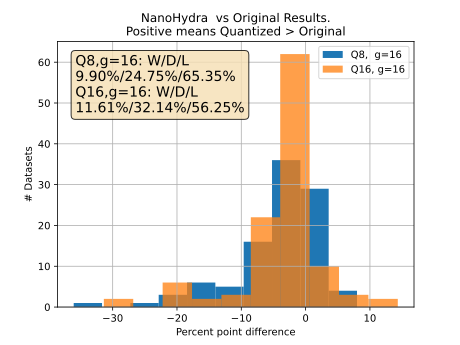
\includegraphics[width=0.75\textwidth]{fig/fig_vs_q_g16_histogram_dev.pdf}
    \caption{Histogram of absolute accuracy deviations of this work to \cite{Dempster2023Hydra} for $g=16$.}
    \label{fig:ucr_hist_vs_q_g16}
\end{figure}
\begin{figure}[h!]
    \centerfloat
    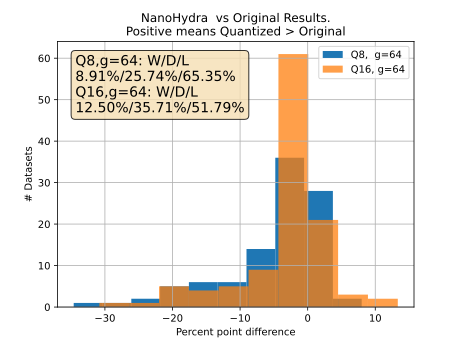
\includegraphics[width=0.75\textwidth]{fig/fig_vs_q_g64_histogram_dev.pdf}
    \caption{Histogram of absolute accuracy deviations of this work to \cite{Dempster2023Hydra} for $g=64$.}
    \label{fig:ucr_hist_vs_q_g64}
\end{figure}

\section{Topological exploration on the ECG5000 Dataset}\label{sec:rs_arch_ecg5000}
In this section, we perform some deeper analysis on the NanoHydra algorithm, by using one of the UCR Datasets as a study case, the ECG5000 dataset.
The ECG5000 dataset consists of 1 second samples of ECG recordings, sampled at 140 Hz, where we have \textbf{five classes}: four types of arrythmias, and the ``No Arrhythmia'' class.
There is a total of 5000 samples, split into 500 training samples and 4500 test samples. This makes it a nice benchmarking dataset, since the heavy imbalance of train/test samples proves an
algorithm's suitability to generalized from a limited test set, and is especially challenging for data-intensive algorithms, favoring those that are stronger one-shot learning capabilities.
Section \ref{sec:rs_acc_topo} presents a study of the influence of the hyperparameters on the prediction accuracy, and Section \ref{sec:rs_gap9_meas} performs
measurements on embedded-targeted metrics using the GAP9 simulator and development board using a selection of two representative algorithm topologies, explained in Table \ref{tbl:gap9_test_cfg}.

\subsection{Hyperparameter influence on accuracy}\label{sec:rs_acc_topo}
Four algorithm topologies, in increasing levels of complexity, are tested against the ECG5000. Figures \ref{fig:vs_g_q16} to \ref{fig:vs_dil_q8} list the hyperparameter configuration used in each of the four topologies.
The data points correspond to the \emph{average} accuracy across \textbf{five} runs of that configuration, and the error bars mark the minimum and maximum accuracy across the five runs for that configuration. In each run, the model
is trained from scratch, and inferred across the test set. The training cycle is extremely fast, as on average we are able to perform a full train+inference cycle in just under 5 seconds, using a CPU and not a GPU. 

\begin{figure}[h!]
    \centerfloat
    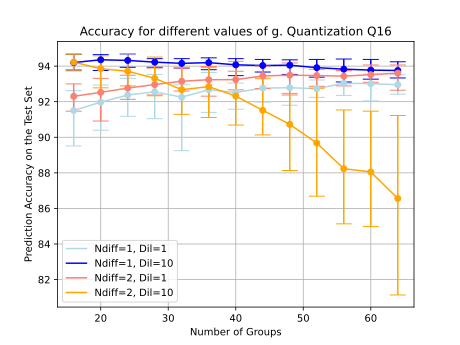
\includegraphics[width=0.75\textwidth]{fig/score_vs_g_q16.pdf}
    \caption{Accuracy of NanoHydra for the ECG5000 dataset across different values of $g$, input quantized in 16-bit. Four topologies considered, in increasing complexity, listed in the legend.}
    \label{fig:vs_g_q16}
\end{figure}
\begin{figure}[h!]
    \centerfloat
    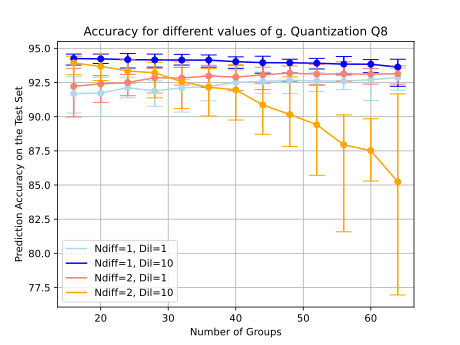
\includegraphics[width=0.75\textwidth]{fig/score_vs_g_q8.pdf}
    \caption{Accuracy of NanoHydra for the ECG5000 dataset across different values of $g$, input quantized in 8-bit. Four topologies considered, in increasing complexity, listed in the legend.}
    \label{fig:vs_g_q8}
\end{figure}
\begin{figure}[h!]
    \centerfloat
    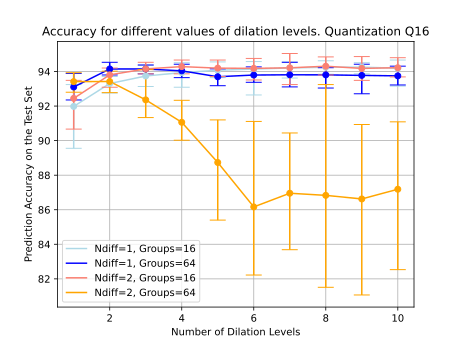
\includegraphics[width=0.75\textwidth]{fig/score_vs_dil_q16.pdf}
    \caption{Accuracy of NanoHydra for the ECG5000 dataset across different dilation levels $N\sb{\text{dil}}$, input quantized in 16-bit. Four topologies considered, in increasing complexity, listed in the legend.}
    \label{fig:vs_dil_q16}
\end{figure}
\begin{figure}[h!]
    \centerfloat
    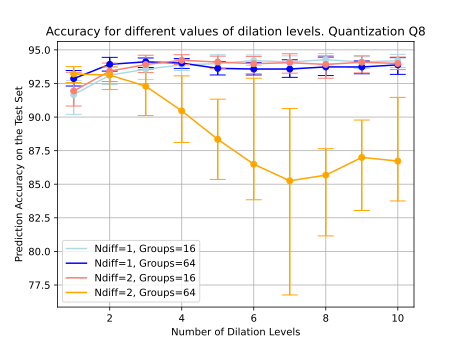
\includegraphics[width=0.75\textwidth]{fig/score_vs_dil_q8.pdf}
    \caption{Accuracy of NanoHydra for the ECG5000 dataset across different dilation levels $N\sb{\text{dil}}$, input quantized in 8-bit. Four topologies considered, in increasing complexity, listed in the legend.}
    \label{fig:vs_dil_q8}
\end{figure}
We can see a few common features in all Figures. The largest model topologies suffer from a decrease in accuracy as the hyperparameter variable increases; furthermore, the spread of accuracies is also very large, representing an absolute swing of almost 15 \% in the worse case.
This represents an interesting feature of this algorithm: \emph{more} is not \emph{better}, and smaller more efficient topologies result in better performing models. 
The explanation is that an increase in the feature vector length can produce a redundant number of features, that are counterproductive in terms of the ability of the classifier to learn.
On the other hand, we note the same effect for excessively \emph{small} models, where the accuracy is lower, but surprisingly not as low as in the excessively large models.
Figures \ref{fig:vs_g_q16} and \ref{fig:vs_g_q8} reveal that, apart from the aforementioned outlier topology, accuracy tends to increase with the number of groups, but this increase tends to show diminishing returns.
We also see that, for the same number of groups, the accuracy is higher when $N\sb{\text{dil}} = 10$ than when $N\sb{\text{dil}} = 1$.
In a first analysis, it might seem that higher $N\sb{\text{diff}}$ tend to produce lower accuracies. 
However, turning our attention to Figures \ref{fig:vs_dil_q16} and \ref{fig:vs_dil_q8}, where the test hyperparameter is, instead, the level of dilations,
we see that the dilation level also has a significant impact on the usefulness of $N\sb{\text{diff}}$, and $N\sb{\text{diff}}$ cannot be analyzed in isolation.
We can see that there is an optimal number of dilations between $2 \leq N\sb{\text{dil}} \leq 4$, and that $N\sb{\text{diff}} = 2$ has a slightly higher accuracy than $N\sb{\text{diff}} = 1$.
Lastly, we can see that the level of quantization of the inputs has limited impact on the accuracy.

\subsection{GAP9 Measurements}\label{sec:rs_gap9_meas}
In this section, we list embedded-specific benchmarks of the NanoHydra model on the ECG5000 dataset. 
In Table \ref{tbl:gap9_test_cfg}, we establish two representative hyperparameter configurations on which we test several variations of the implementation.
These configurations were chosen in accordance to the observations of Section \ref{sec:rs_acc_topo}, so that we have two design points of similar accuracy but one is approximately
a third the size of the other. This can be seen in terms of the memory requirements per computation stage in Table \ref{tbl:gap9_test_cfg_reqmem}, and in terms of number of millions of
multiply-accumulate operations in Table \ref{tbl:gap9_test_cfg_reqcomp}. In Table \ref{tbl:gap9_inf_results} we present inference benchmarks of the configurations listed before, with some
variations, namely different levels of quantization of the input (8-bit or 16-bit) implying that different levels of SIMD are used (2-way or 4-way, respectively), which has an impact
in the inference time. Each design configuration was trained 20 times in the development PC, the weights of the most accurate model were deployed to the GAP9 simulator/board where they were inferred 20 times,
across which the total number of cycles was averaged. The inference time assumes a clock speed of 100 MHz.

\begin{table}[p!]
    \centerfloat
    \rowcolors{2}{lightgray}{white}
    \begin{tabular}{ c c c c c c c }
    \toprule
    \textbf{Configuration Name} & $N\sb{\text{diff}}$ & \textbf{Kernels Per Group} & \textbf{Groups} & $N\sb{\text{dil}}$ \\
    \midrule
    CFGA & 1 & 8 & 16 & 3 \\
    CFGB & 2 & 8 & 16 & 5 \\
    \bottomrule
    \end{tabular}
    \caption{NanoHydra configurations used on the ECG5000 dataset tests on the GAP9}%
    \label{tbl:gap9_test_cfg}
\end{table}

\begin{table}[p!]
    \centerfloat
    \rowcolors{2}{lightgray}{white}
    \begin{tabular}{ c c c c }
    \toprule
    \textbf{Configuration Name} & Kernels (Step 1) & Classifier (Step 2 \& 3) & Activations \\
    \midrule
    CFGA & 0.070 kB &  3 kB & 0.75 kB \\
    CFGB & 0.070 kB & 10 kB & 2.5  kB \\
    \bottomrule
    \end{tabular}
    \caption{Memory requirements for the trainable parameters and activations in the different configurations of NanoHydra, in kB}%
    \label{tbl:gap9_test_cfg_reqmem}
\end{table}

\begin{table}[p!]
    \centerfloat
    \rowcolors{2}{lightgray}{white}
    \begin{tabular}{ c c c }
    \toprule
    \textbf{Configuration Name} & Kernels (Step 1) & Classifier (Step 2 \& 3)\\
    \midrule
    CFGA & 2.88  & 0.0064 \\
    CFGB & 0.864 & 0.00192 \\
    \bottomrule
    \end{tabular}
    \caption{Computational requirements for the trainable parameters and activations in the different configurations of NanoHydra, in MMACs}%
    \label{tbl:gap9_test_cfg_reqcomp}
\end{table}

\begin{table}[p!]
    \centerfloat
    \rowcolors{2}{lightgray}{white}
    \begin{tabular}{ c c c c c c c c}
    \toprule
    \textbf{Quantz.} & \textbf{Config} & \textbf{Parallel} & \textbf{Accuracy} & \textbf{MCycles} & \textbf{Inf. Time} & \textbf{Inf. Energy} & \textbf{Train Time} \\
    \midrule
    Q16 & CFGA & Yes & 94.38\% & 0.1312 & 1.312 ms & 15.85 \mu J & 38 s\\
    Q16 & CFGB & Yes & 94.67\% & 0.4184 & 4.189 ms & 51.14 \mu J & 95 s\\
    Q8  & CFGA & Yes & 94.13\% & 0.0956 & 0.956 ms & 14.22 \mu J & 38 s\\
    Q8  & CFGB & Yes & 94.47\% & 0.2990 & 2.990 ms & 38.32 \mu J & 95 s\\
    Q16 & CFGA & No  & 94.38\% & 0.7162 & 7.162 ms & 63.43 \mu J & 38 s\\
    Q8  & CFGA & No  & 94.13\% & 0.4823 & 4.823 ms & 42.15 \mu J & 38 s\\
    \bottomrule
    \end{tabular}
    \caption{Inference Results of the ECG5000 dataset on the GAP9. Results presented correspond to the average of 20 inference rounds. The reported accuracy is the maximum across the training rounds, the train time is the total time of all 20 training rounds.}%
    \label{tbl:gap9_inf_results}
\end{table}
The accuracy of all design points is above 94 \%, and the absolute difference between the most and least accurate is as low as 0.5\%. 
The effect of increasing the quantization level from 16-bit to 8-bit consistently lowers the accuracy, but by only a mere 0.2\%, while at the same time substantially speeding up the inference time by 40\%.
Parallelization has no impact on accuracy, as the model is still the same, only compiled without parallelization enabled. Parallelization seems to consistently speed up the computations by \~5.5x, instead of the theoretical maximum of 8x. 
The discrepancy is explained by two factors. First, the parallel section incurs on the small additional overhead of copying-in and copying-out the operands. Second, we are only parallelizing Step 1, which although accounts
for roughly 99 \% of the MAC operations as explained in Section \ref{tbl:im_nanohydra_rel_eff}, this is not directly translated into inference time, since they are also only a fraction of the type of computations performed inside Step 1.
If instead we consider that Step 1 makes up 94 \% of the computational time, then according to Amdahl's law 

\begin{equation}
s = \frac{1}{(1-f) + \frac{f}{p}}
\end{equation}
which allows us to calculate the speed-up $s$ that we get by parallelizing a fraction $f$ of the computation time by $p$ processors,
we get that $s \approx 5.6$ when $f=0.94$ and $p=8$, as is the case in our situation.

Lastly, a word should be given about the training time. We remarkably take only $95 / 20 \approx 4.75$ seconds to train the most accurate model, without using any GPU, but only a CPU.
Using this model is energy-efficient not only in the embedded MCU at inference time, but also during training at the PC Workstation, since not only CPUs consume less power than GPUs
\footnote{The model was trained in an AMD Ryzen9 5900X CPU, which has a TDP of 105W. For instance, a Nvidia RTX 4090 GPU has a TDP of 450W}, the model only draws power for $\approx5$ seconds during each training round. 

\subsection{Comparison to Related Work}

\section{Multichannel NanoHydra for KWS}\label{sec:rs_speechcomms}
Hydra as formulated in \cite{Dempster2023Hydra} supports only single channel time series data.
In fact, some types of time-series data has more than one channel. This is the case for audio data, for instance.
In KWS tasks, for instance, we generally transform the input audio signal with MFCC, generating several streams of spectral samples across time.
Towards the purpose of using MFCC transforms to use as input to a KWS classifier, we expanded the capabilities of Hydra by simply
repeating the RCK transform for all MFCC channels, and concatenating the output from all channels in our feature vector.
The proposed change was performed, and the experiment settings were the following:

\begin{itemize}
    \item \textbf{Data Augmentation} - Augment underrepresented classes such that we end up with roughly the same number of training 
                                       samples per class ($2\times$ 'Unknown' class, $80\times$ 'Silence' class, $15\times$ all others).
                                       The augmentation techniques were two: time-shift the samples by an amount uniformly sampled from the interval [-150ms, 150ms]; add a random noise sample from the 'Silence' class, with volume scaling uniformly sampled from the interval [0, 0.15].
    \item \textbf{MFCC Transform} - window length of 512 samples, hop length of 128. The FFT length is 512 samples long and the maximum frequency set to the Nyquist frequency of 8000Hz. We select the 8 lowest MFCC channels.
    \item \textbf{NanoHydra Transform} - $N\sb{\text{diff}} = 2$, $N\sb{\text{dil}} = 2$, $k=8$ and $g=32$
\end{itemize}
The initial results were not very convincing. We started by running Hydra on the raw waveform, but that yielded accuracies in the range of 60\%. The introduction of the MFCC transform and data augmentation improved the prediction
accuracy substantially, by bringing it over the 80\% mark. However, the accuracy still would not improve with increased model size or with the tuning of hyperparameters. Looking again at how NanoHydra works, one can
see that this model \textbf{accumulates} the statistics of the patterns it detects. This is a problem, in the sense that the after/before speech areas of the sample would ``pollute'' these statistics with non-signal information.
Therefore, we implemented a mechanism that sets to zero the MFCC channels whenever the signal power (approximated by the lowest MFCC channel) is lower than a given threshold. This yielded a significant improvement, increasing the
prediction accuracy up to 85\%. Lastly, normalizing the MFCC channels on a per-channel basis yielded another substantial improvement up to close to 89\%. When such a normalization procedure is in place, the lowest MFCC channel threshold
used is zero, and our experiences have shown that any value lower or higher does not improve prediction accuracy. These changes made NanoHydra usable, achieving an acceptable, but slightly far from SOTA prediction accuracy. They are a substantial
contribution to how Hydra/NanoHydra can be used in KWS problems, and serve as a basis for future work.

The accuracy results, along with the comparison to related work, are shown in Table \ref{tbl:rs_speechcomms}


\subsection{Comparison to Related Work}
As we can see, the NanoHydra results on the Google Speech Commands dataset, although still within the 
acceptable range, are not competitive with other published architectures that achieve higher prediction accuracies, while
still having faster and more compact models. A large design exploration has been 
\begin{table}
\centerfloat
\rowcolors{2}{lightgray}{white}
    \begin{tabular}{ c c c c c c c c}
    \toprule
    Reference & Model & Test Accuracy & Memory & Ops & Year & Citation & Reproducible? \\

    \midrule
    \cite{Zhang2017}   &        DS-CNN & 94.4\% & 38.6 kB & 5.4M & 2017 & 483 &  \href{https://github.com/ARM-software/ML-KWS-for-MCU}{Yes} \\
    \cite{Andrade2018} &       Att-RNN & 96.9\% &  202 kB &   ?? & 2018 & 113 &  Yes \\
    \cite{Tang2018}    &       ResNet8 & 94.1\% &  110 kB &  30M & 2018 & 241 &  \href{https://github.com/castorini/honk/}{Yes} \\
    \cite{Tang2018}    & ResNet-Narrow & 90.1\% & 19.9 kB & 5.7M & 2018 & 241 &  \href{https://github.com/castorini/honk/}{Yes} \\
    \cite{Jansson2018} &    ConvNetRaw & 89.4\% &  700 kB &   5M & 2018 &  19 &  No \\
    \textbf{Ours}      &     NanoHydra & 88.7\% & 56.1 kB & 2.6M & 2024 & n/a &  Yes \\
    \bottomrule
\end{tabular}
\label{tbl:rs_speechcomms}
\caption{Comparison of the Google Speech Commands inference benchmarks with related work}
\end{table}

\section{Current limitations}
The main current limitation of NanoHydra is its limited accuracy in the Google Speech Commands dataset. The multichannel architecture we propose seems to greatly benefit from the MFCC transform, 
but future potential improvements could be achieved -- not only in this specific dataset, but in other multichannel datasets -- by increasing the dimensionality of the receptive field.
The approach of this work is to repeat the transform on a per-channel basis, but this implies that the inter-channel patterns and dependencies are not extracted in the convolutional transforms.
This could be achieved, for instance, by making the randomized kernels to operate as a matrix block, in a fashion similar to that of CNNs.